%
%          MANUSCRIPT STARTS HERE
%
%%%%%%%%%%%%%%%%%%%%%%%%%%%%%%%%%%%%%%%%%%%%%%%%%%%%%%%%%%%%%%%%%%%%%%%%%%
\documentclass[]{MathAppl18}
%Polish letter codding
\usepackage[OT4,T1]{fontenc}
\usepackage[utf8]{inputenc}
\usepackage{polski}
\usepackage{graphicx}
\usepackage{wrapfig}

\usepackage{xcolor}

\usepackage{amsmath}
\usepackage{amssymb}
\usepackage{filecontents}

% Cyrylica
%\input cyracc.def
%\newcommand\cyrfamily{\fontencoding{OT2}\fontfamily{wncyr}
%\selectfont\cyracc}
%\DeclareTextFontCommand{\textcyr}{\cyrfamily} 
%\volume{46}
\usepackage[english,polish]{babel} %PS
\usepackage{lastpage} %PS

\usepackage{etex} %PS

\usepackage{color} 
\usepackage{cite} %PS
%\usepackage{here} %PS

\RequirePackage[numbers]{natbib}
\renewcommand{\bibsection}{}
%\usepackage[cam,a4,center]{crop}suppress this lines.
\usepackage[colorlinks=true]{hyperref}
%\usepackage{hyperref}
  \hypersetup{
    pdftitle={Teplate Mathematica Applicanda }, %%<--To wymieni? 
    pdfauthor=Nowy Autor, %%<--TO wymieni?
    colorlinks,
    urlcolor=blue,
    filecolor=magenta,
    citecolor=green, 
    linkbordercolor={1 1 1}, % set to white
    citebordercolor={1 1 1},  % set to white
    urlbordercolor={ 1 1 1}  % set to white
  } 
 \RequirePackage[hyperpageref]{backref} 
    \renewcommand*{\backref}[1]{}  
    \renewcommand*{\backrefalt}[4]{
       \ifcase #1 
          No cited.
       \or
          cited on p. #2.
       \else
          cited on pp. #2.
       \fi}  
\newcommand{\orcid}[1]{\href{https://orcid.org/#1}{
\includegraphics[scale=.05]{orcid.png}}}	
\newcommand{\orcidcode}[1]{\href{https://orcid.org/#1}{#1}}
       
\def\repo{http://wydawnictwa.ptm.org.pl/index.php/matematyka-stosowana/article/viewArticle}  
\newcommand*{\eudml}[1]{\href{http://eudml.org/doc/#1}{#1}} 
 %<http://eudml.org/doc/209100>

%
%\newcommand*{\doi}[1]{\href{http://dx.doi.org/#1}{doi: #1}}
%\newcommand*{\MR}[1]{\href{http://www.ams.org/mathscinet-getitem?mr=#1&return=pdf}{#1}}
%\newcommand*{\ZBL}[1]{\href{http://www.zentralblatt-math.org/zmath/en/advanced/?q=an:#1&format=complete}{Zbl #1}}
%\newcommand*{\ZBLid}[1]{\href{https://zbmath.org/?q=ai:#1}{ZBLid:#1}}   %%<-definicja KSz
%\newcommand*{\JFM}[1]{\href{http://www.zentralblatt-math.org/zmath/en/advanced/?q=an:#1&format=complete}{JFM #1}}

%\newcommand*{\eLIBru}[1]{\href{https://elibrary.ru/item.asp?id=#1}{eLibrary.ru #1}}
\pdfoutput=1
\pdfcompresslevel=0
\usepackage{graphicx}
\usepackage{wrapfig}
\graphicspath{{./Figures/},{./Pictures/}}
\usepackage{multicol}
%%%%%%%%%%%%%%%%%%%%%%%%%%%%%%%%%%%%%%%%%%%%%%%%%%%%%%%%%%%%%%%%%%%%%%%
%%                    Submission information - GLOBAL                %%
%%                      Inserted by editor                           %%
%%%%%%%%%%%%%%%%%%%%%%%%%%%%%%%%%%%%%%%%%%%%%%%%%%%%%%%%%%%%%%%%%%%%%%%
\firstpage{i}    
%www
\LogoG{
\includegraphics[width=0.18\textwidth]{ma.png}}
\volume{46}
\fasc{2}
\years{2018}
%MS
\LogoGMS{
\includegraphics[width=0.18\textwidth]{ms.png}}
\volumeMS{26}
\numberMS{63}
%\wwwfalse
\wwwtrue
% LOCAL DEFINITINS
%+==============================
%\newtheorem{thm}{Theorem}[section]
%\newtheorem{cor}[thm]{Corollary}
%\newtheorem{lem}[thm]{Lemma}
%\newtheorem{prob}[thm]{Problem}
%\newtheorem{ass}[thm]{Assumption}

%% A numbered theorem with a fancy name:

%\newtheorem{mainthm}[theorem]{Main Theorem}

%% Numbered objects of "non-theorem" style (text roman):

%\theoremstyle{definition}
%\newtheorem{defin}[theorem]{Definition}
%\newtheorem{rem}[theorem]{Remark}
%\newtheorem{exa}[theorem]{Example}
%+====================================================
%\tpauthortrue % PS11lis12
%%%%%%%%%%%%%%%%%%%%%%%%%%%%%%%%%%%%%%%%%%%%%%%%%%%%%%%%%%%%%%%%%%%%%%%
%%                    Submission information                         %%
%%                      Inserted by editor                           %%
%%%%%%%%%%%%%%%%%%%%%%%%%%%%%%%%%%%%%%%%%%%%%%%%%%%%%%%%%%%%%%%%%%%%%%%
\secnameMS{MATHEMATICS FOR SOCIAL AND ART SCIENCES}
\pages{193--206}
%\receivedPL[3 wrze?nia 2014]{ 26 listopada 2012}
\received[5th of June 2017]{ 11th of January 2017}
\lastrevision{}
\logo{}{}{}%Do not change 9 above lines
\def\doinum{10.14708/ma.v43i1.xxx}%% http://wydawnictwa.ptm.org.pl/index.php/matematyka-stosowana/article/view/614
%Do not change 9 above lines

%%Preliminaries
%%Preliminaries
\title{A novel semiparametric model for hydrogen-deuterium exchange monitored by mass spectrometry data.}
%\dedicated{Dedicated to ....}

%\dedicated{Dedicated to ....}

%\tpauthorfalse % PS11lis12
\tpauthortrue % PS11lis12
%%The First author




\author[K, Grzesiak]{Krystyna Grzesiak\orcid{0000-0003-2581-7722}}
\thanks{This research was financed by the Foundation of Polish Science (TEAM TECH CORE FACILITY/2016-2/2 Mass Spectrometry of Biopharmaceuticals - improved methodologies for qualitative, quantitative and structural characterization of drugs, proteinaceous drug targets and diagnostic molecules) to Michał Dadlez.}

\affiliation{University of Wroc{\l}aw}
\address{Faculty of Mathematics and Computer Science, University of Wroc{\l}aw, Fryderyka Joliot-Curie 15, 50-383 Wrocław}
\email{krygrz11@gmail.com}
\city{Wroc{\l}aw}


\author[W. Puchała]{Weronika Puchała\orcid{0000-0003-2163-1429} \footnotemark[1]}

\affiliation{Polish Academy of Sciences}
\address{Institute of Biochemistry and Biophysics, Polish Academy of Sciences, FAdolfa Pawińskiego 5A, 02-106 Warszawa}
\email{puchala.weronika@gmail.com}
\city{Warszawa}


\author[M. Dadlez]{Michał Dadlez\orcid{0000-0001-8811-5176} \footnotemark[1]}

\affiliation{Polish Academy of Sciences}
\address{Institute of Biochemistry and Biophysics, Polish Academy of Sciences, FAdolfa Pawińskiego 5A, 02-106 Warszawa}
\email{michald@ibb.waw.pl}
\city{Warszawa}


\author[M. Bogdan]{Małgorzata Bogdan\orcid{0000-0002-0657-4342}}

\affiliation{University of Wroc{\l}aw}
\address{Faculty of Mathematics and Computer Science, University of Wroc{\l}aw, Fryderyka Joliot-Curie 15, 50-383 Wrocław}
\email{malgorzata.bogdan20@gmail.com }
\city{Wroc{\l}aw}


\author[M. Burdukiewicz]{Michał Burdukiewicz\orcid{0000-0001-8926-582X} \footnotemark[1]}

\affiliation{Medical University of Bialystok}
\address{Jana Kilińskiego 1, 15-089 Bia{\l}ystok}
\city{Bia{\l}ystok}
\email{michalburdukiewicz@gmail.com}

\subjclass[2010]{Primary: 62J05; Secondary: 92D20}
\keywords{deuterium uptake, hydrogen-deuterium exchange, mass spectrometry, HDX-MS, semiparametric model, spline regression}

\begin{document}
\vspace{-5ex}

\setcounter{page}{193} 
\selectlanguage{english}\Polskifalse

\begin{abstract}
%During the incubation in heavy water (D2O) more exposed residues undergo the exchange of amide hydrogens to deuters much faster than others. The measurements of peptides' masses reveal the stability of the hydrogen bonding network and regions of protein with limited solvent accessibility. The speed of the exchange may depend on the biological state (e.g. with or without a present ligand) i.e. can be related to the changes of the conformation of their structure.
The hydrogen-deuterium exchange monitored by mass spectrometry (HDX-MS) is one of the methods for studying the structure of proteins. HDX-MS associates the speed of hydrogen-deuterium exchange with the regional stability of a protein. Such stability is affected by the biological state (e.g., presence of a biological ligand or lack thereof). Therefore, the changes in the protein's molecular structure caused by the biological state are inferred from the differences in the speed of hydrogen-deuterium exchange. In the following paper, we propose a test based on a mixed semiparametric model and ridge regression that allows for the accurate identification of regions with significantly different exchange speeds at two biological states. To assess its performance, we compared it with existing HDX-MS data analysis methods.\end{abstract}

\section{Introduction}

Proteins are common biomolecules facilitating many biological processes such as transport (e.g transport of oxygen, iron), catalysts (hydration of carbon dioxide), storage (ferritin stores iron ions in the liver), and many others. The structure of a protein in its most fundamental level is a chain of amino acid residues bonded by so-called peptide bond. However, in the process known as folding, this chain assumes different spatial structures. It is commonly assumed that the protein's function is usually defined by its structure~\citep{anfinsen1972formation}. %The experimental data suggest that the proteins can have both regions essential for their functioning and regions that may be excised without any impact on their functionality. 
Thus, to understand how proteins participate in biological process, we need to examine their structures. 

The hydrogen-deuterium exchange monitored by mass spectrometry (HDX-MS) recently emerged as a tool for the assessment of protein structure and related properties including flexibility, stability, and affinity towards various interacting compounds, i.e. ligands and other macromolecules. This technique can measure the structural alterations caused by a biological state, an umbrella term for factors ranging from the presence of interacting molecules to the environmental conditions~\citep{masson2019recommendations}. %which is represented by the protection of amino acid residues as described in . 

To do so, the proteins in different biological states are incubated in heavy water (D$_2$O) for a certain time. Less protected amino acid residues (e.g., more exposed to the solvent) are undergoing the exchange of hydrogens to deuters much faster than better-protected residues~\citep{BERGER1957106}. The most common approach to HDX-MS does not rely on measuring the mass of the whole protein, but rather its short fragments, peptides. Since the mass of deuterium is twice the size of hydrogen's, the differences in the masses of peptides allow of the comparison of the protection of given residues along the protein for different biological states. 
% usunac sprayer
%Next, the deuterated protein chain is cut into shorter fragments called peptides. They can be of various lengths and might partially overlap each other. Having a protein cut into peptides the experimenter provides charge using a sprayer. The charge is added randomly and specifics about its value are provided based on a flight track inside a spectrometer. Thus, one usually has few measurements of one peptide with different charges and aggregates results within one replication afterward. The procedure described above is shown in the figure \ref{HDX}.

% \begin{figure}[h!]
%    \centering
%    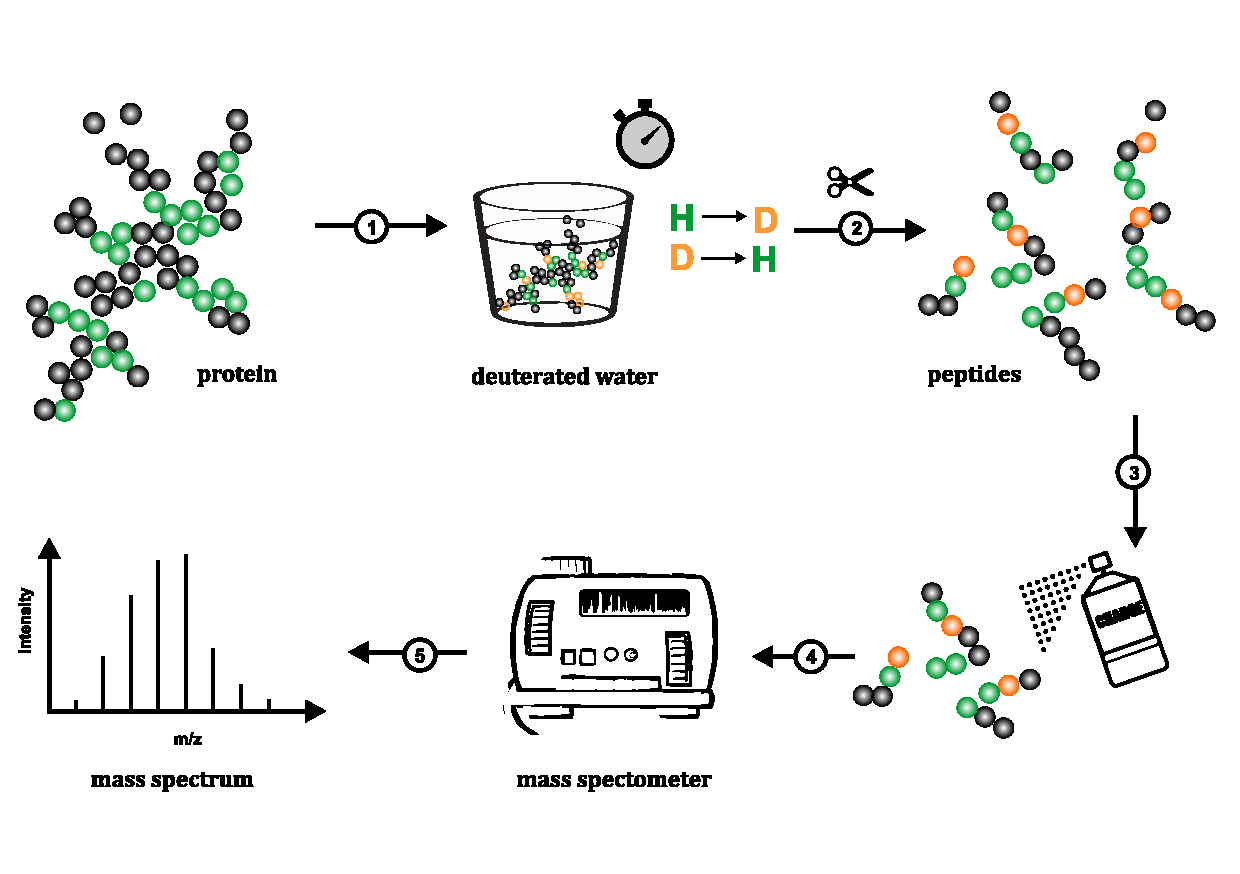
\includegraphics[width=0.7\textwidth]{Figures/hdx.pdf}
%    \caption{Hydrogen - deuterium exchange monitored by mass spectrometry \label{HDX}}
%\end{figure}
The HDX experiments are said to be monitored by mass spectrometry as the mentioned masses are calculated based on mass spectra - an intensity versus mass-to-charge ratio ($m/z$) plots representing the distribution of ions (the occurrence of given $m/z$ value). From the spectrum, we calculate a centroid which is identified as a measurement of the peptide mass after deuteration~\citep{10.1093/bioinformatics/btaa587}. The difference between the masses before and after exposure to D$_2$O is called deuterium uptake. The measurements of deuterium uptake are made for several exposure times and repeated within several replications. A deuterium uptake curve is a longitudinal study of deuterium uptake over time for a single peptide at a given biological state.



\paragraph{HDX data analysis} 

This paper concerns the problem of the inference about the structural (protection) factors of the peptides, based on their masses during the measurement. The challenge is to identify peptides whose deuterium uptake differ significantly between biological states. Such differences imply that biological state affects the structure of peptide's source region in the protein. The testing problem can be written down using the following hypotheses:
\begin{center}
    \textit{$H_0$: The deuterium uptake does not differ between states}\\
    vs.\\
    \textit{$H_1$: The deuterium uptake differs between states.}
\end{center}

\section{Semiparametric test}


We propose a novel test based on a semiparametric mixed model regularized by ridge regression for HDX-MS data. The test is meant for a specifically designed experiment in which each replication was a sample prepared by incubation of the protein stock (at a particular biological state) in the labeling solution for various time-points i.e. 0s (control), 10 s, 60 s, etc. Thus, under the term \textit{replication} we understand a single deuterium uptake curve.

The model requires the following data:
\begin{itemize}
    \item deuterium uptake (response) - calculated from spectrum
    \item Exposure time
    \item Biological state
    \item Replication ID
\end{itemize}
We describe the testing procedure applied in the semiparametric test in detail in four steps:

\paragraph{Step 1: Regression spline}

The regression spline is an extension of the linear approach that allows for nonlinear relationship between response and the features \citep[see][Generalized Additive Models]{huang2014introduction}. Such a model for the response $Y$ along with predictors $X_1, \ldots, X_p$ can be represented by the following formula
\begin{equation}
    \label{semi_model1}
    y_i = \beta_0 + \sum_{j = 1}^p f_j(x_{ij}) + \epsilon_i ,
\end{equation}
where $f_j$, $j = 1, \ldots, p$ are smooth (nonlinear) functions. The semiparametric part of our model is a spline based on the simplest base functions $f$, so called truncated lines \citep[see][]{https://doi.org/10.1002/sim.1991}. Namely, for $y$ denoting deuteration level and $x_T$ denoting exposure time we have 

\begin{equation}
\label{spline_fun}
    y_i = \beta_0 + \beta_1 x_{Ti} + \sum_{k = 1}^{K} u_k (x_{Ti} - \kappa_k)_+.
\end{equation}
where $u_k$ for any $k = 1, \ldots, K$ are coefficients corresponding to $k^{th}$ truncated line (exposure time) and for any $x, a \in \mathbb{R}$ we define  $$(x - a)_+ = \max(0, ~x - a).$$
We create the design matrix $\mathbf{X}$ for all the time points as follows
$$
\mathbf{X} = \begin{pmatrix}
(x_1 - \kappa_1)_+ & \hdots & (x_1 - \kappa_K)_+\\
\vdots & &\vdots \\
(x_n - \kappa_1)_+ & \hdots & (x_n - \kappa_K)_+
\end{pmatrix}
$$
and go to step 2.


\paragraph{Step 2: Regularization by ridge regression}

We use $l_2$-norm penalized regression to select columns of $\mathbf{X}$. To do so, we fit the ridge regression model with response $Y$ (deuterium uptake) and the abovementioned design matrix $\mathbf{X}$, by solving the formula  \citep[Shrinkage Methods]{hastie01statisticallearning}

\begin{equation}
\label{ridge}
    \hat{\beta}_{ridge} = \underset{b \in \mathbb{R}^p}{\arg\min}~\bigg\lbrace||Y - Xb||^2 + \lambda \sum_{i = 1}^p b_i^2\bigg\rbrace
\end{equation}
where $\lambda$ is the regularization penalty. Let us notice that the greater value of $\lambda$ we set, the sparser estimator of $\beta$ we obtain. At the same time, the sparser estimator of $\beta$ we get, the fewer knots we select to the spline and the more 'boxy' the target model will be as shown on the figure 1.
 \begin{figure}[h]
    \centering
    \label{knots}
    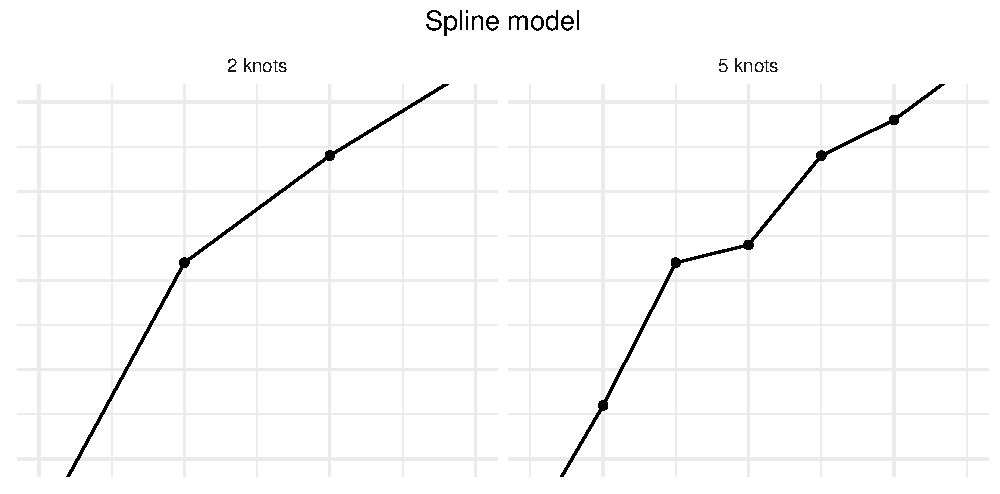
\includegraphics[width=0.8\textwidth]{Figures/plot_spline.pdf}
    \caption{Splines depending on the number of knots.}
\end{figure}
We denote the set of chosen knots (time points) as $\kappa_{ridge}$, and consequently the semiparametric part of the model as 
$$\sum_{\kappa \in \kappa_{ridge}} u_\kappa (x_{Ti} - \kappa)_+$$
and go to step 3.

\paragraph{Step 3: Final model}

The starting point of our model is a simple linear model with an interaction term proposed in \citep{liu2011hdx}

\begin{equation}
\label{final3}
    y_i =  \beta_0 + \beta_T x_{Ti} + \beta_S x_{iS} + \beta_{TS}x_{Ti}x_{Si}+ \epsilon_i
\end{equation}
where $x_S$  denotes protein state. Since the considered data has a longitudinal characteristic, it is desirable to fit a model with random effects \citep[see][]{10.1093/ansci/1973.Symposium.10}. Our model includes two random intercepts - one varying across different curves ($b_{id}$) and second across different time points ($b_T$). Next, we add penalized semiparametric part and obtain the final model:

\begin{equation}
\label{final3}
    y_i =  \beta_0 + b_{id} + b_{T}  + \beta_T x_{Ti} + \beta_S x_{iS} + \beta_{TS}x_{Ti}x_{Si}+ \sum_{\kappa \in \kappa_{ridge}} u_\kappa (x_{Ti} - \kappa)_+ + \epsilon_i.
\end{equation}


\paragraph{Step 4: Testing}

Comparing the differences in deuteration levels in the case of the model-based approaches comes down to determining whether the state indicator is dependent on the measurement of masses. In other words, we test whether the variable describing the protein state should be selected for the model. It can be done via the F test in the context of nested models comparison. In the case of comparing the fixed parts of mixed models, we use the analogous version of the F-test extended by Satterthwaite's method for computing the denominator degrees of freedom and F-statistics~\citep{kuznetsova2017lmertest}. %The method is available in the R-package $lmerTest$ as it provides us with the method $anova$ for mixed models.


\section{Simulation}

We simulated the data of $73$ peptide sequences using the R-package \textit{powerHaDeX} (available on CRAN \citep{powerHaDeX}). A single data set consists of $4$ replications of the experiment and two biological states. Thus, there are $24$ different deuterium uptake curves. The measurements of deuterium uptake were collected at the exposure times 5, 10, 20, 30, 40, 50, 60, 100, 300, 500, 900, 1200, 1500, 1800, 2100, 2400, 3600, 7200, 21600, 43200 in seconds (Figure~3). 
 \begin{figure}[h]
    \label{combined_data}
    \centering
    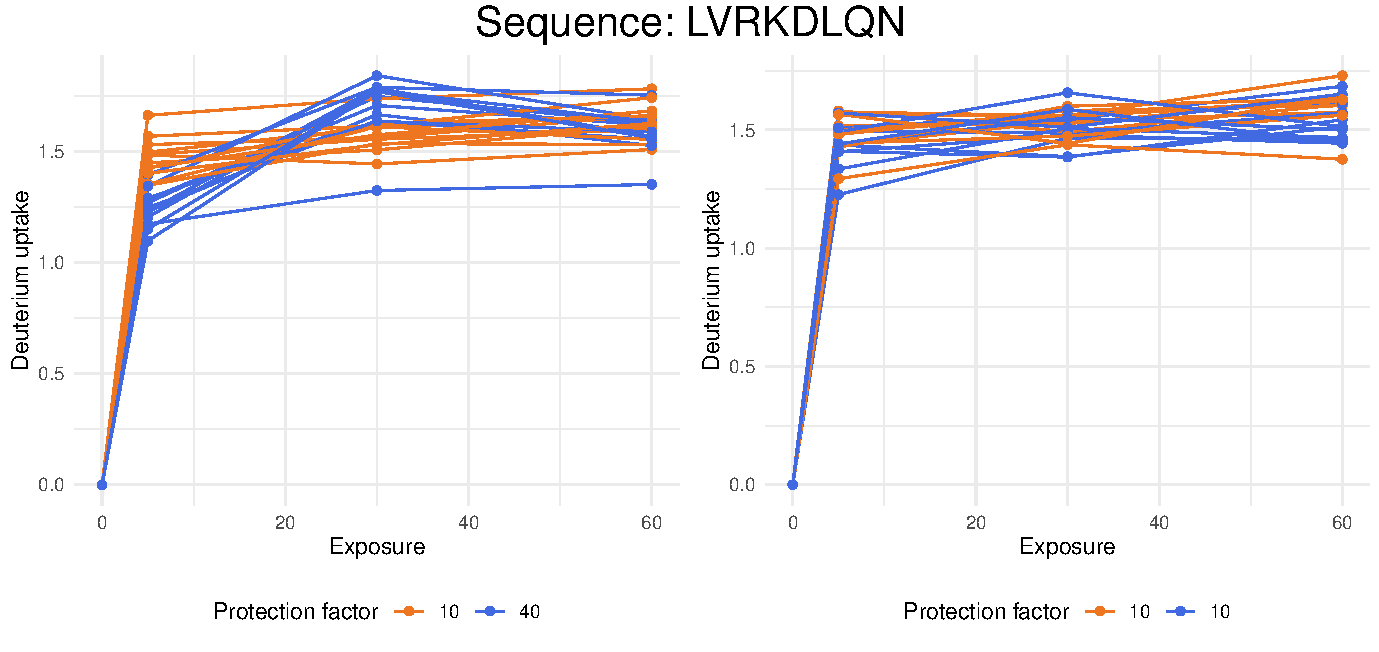
\includegraphics[width=1\textwidth]{Figures/plot_curves.pdf}
    \caption{An example testing data set}
\end{figure}
 
 The simulated data covers two cases. The first happens when we deal with different values of the protection factor, i.e. when the null hypothesis is false and the rejections are true discoveries (the plot on the left). The second is when the protection factors are equal between groups and the null hypothesis is true (the plot on the right). Then, the rejections are false discoveries (type I errors).

\section{Results}
The outcome of our simulation is the set of rejection rates in the pairwise testing procedure at the significance level $0.05$ presented on three charts. Each of them is composed of a grid of average rejection rates depending on the considered hypothesis. On the grid's diagonal (in black frames) the null hypotheses are true ($Pf_1 = Pf_2$) so the rejection rate is the estimator of type I error. Beyond the diagonal, the null hypotheses are false ($Pf_1 \neq Pf_2$) so the rejection rate is the estimator of power. The three following cases are presented on the figure 3:
\begin{itemize}
    \item Plot 1: small values of $\Delta Pf$, $Pf_1$, $Pf_2$,
    \item Plot 2: small values of  $\Delta Pf$ and great values of $Pf_1$ and $Pf_2$,
    \item Plot 3: great values of  $\Delta Pf$.
\end{itemize}

We have also included in our comparison three tests addressing the same hypothesis:

\begin{itemize}
    \item HDX-Analyzer model \citep{liu2011hdx} - models jointly the effect of time and protein state by including regression terms for both quantities and an interaction term
    \begin{equation}
    \label{deuteros}
        y_i = \beta_0 + \beta_T x_{iT} + \beta_S x_{iS} + \beta_{TS}x_{iT}x_{iS} + \epsilon_i.
    \end{equation}
    

    \item MEMHDX mixed model \citep{10.1093/bioinformatics/btw420} - linear mixed model including the effect of a replication:
     \begin{equation}
        y_{i, r} = \beta_0 + \beta_T x_{iT} + \beta_S x_{iS} + \beta_{TS}x_{iT}x_{iS} + w_{i,r} + \epsilon_i,
    \end{equation}
    where $w_r$ is a random effect associated with the replication $r$.
    
    
    \item Houde's confidence intervals test \citep{houde2011utility} - community recognized test derived based on an empirical evaluation of a dataset collected by the author.
\end{itemize}

\paragraph{Type I error}

We discuss the results starting with the type I error. As we can see on the figure 3 the Houde's test turns out to be conservative when compared to the others. The null hypothesis is rejected by Houde's test on average in $1\%$ of the cases. However, the other approaches do not fall far behind. The models HDX-Analyzer and MEMHDX generally hold the type I error at $5\%$ level and model fitted after variable selection done by ridge regression mostly reaches $6\%$ of false rejections.

\paragraph{Power}

The main remark that we can notice first is that in case of small differences between the protection factors all the tests have trouble with accurate rejections. It is not surprising, as for close protection factors we obtain close exchange probabilities, and consequently, close deuteration levels. Thus, such a situation requires a big sensitivity of the test. Since even a small change of the protection factor affects the whole protein regarding its conformation and dynamics we are interested in finding a test as sensitive as it is possible, which is kind of a challenge while keeping the type I error at a small level.

As we can see on the first plot, in the case of small values of $Pf_1$ and $Pf_2$ the test based on the spline model reaches on average better power when compared to the existing tools. When $\Delta Pf$ is small, the existing methods have a way lower rate of true rejections, except for Houde's intervals. The results of Houde's test are better but still differ from the semiparametric model. 

\begin{figure}[h!]
\label{results}
    \centering
    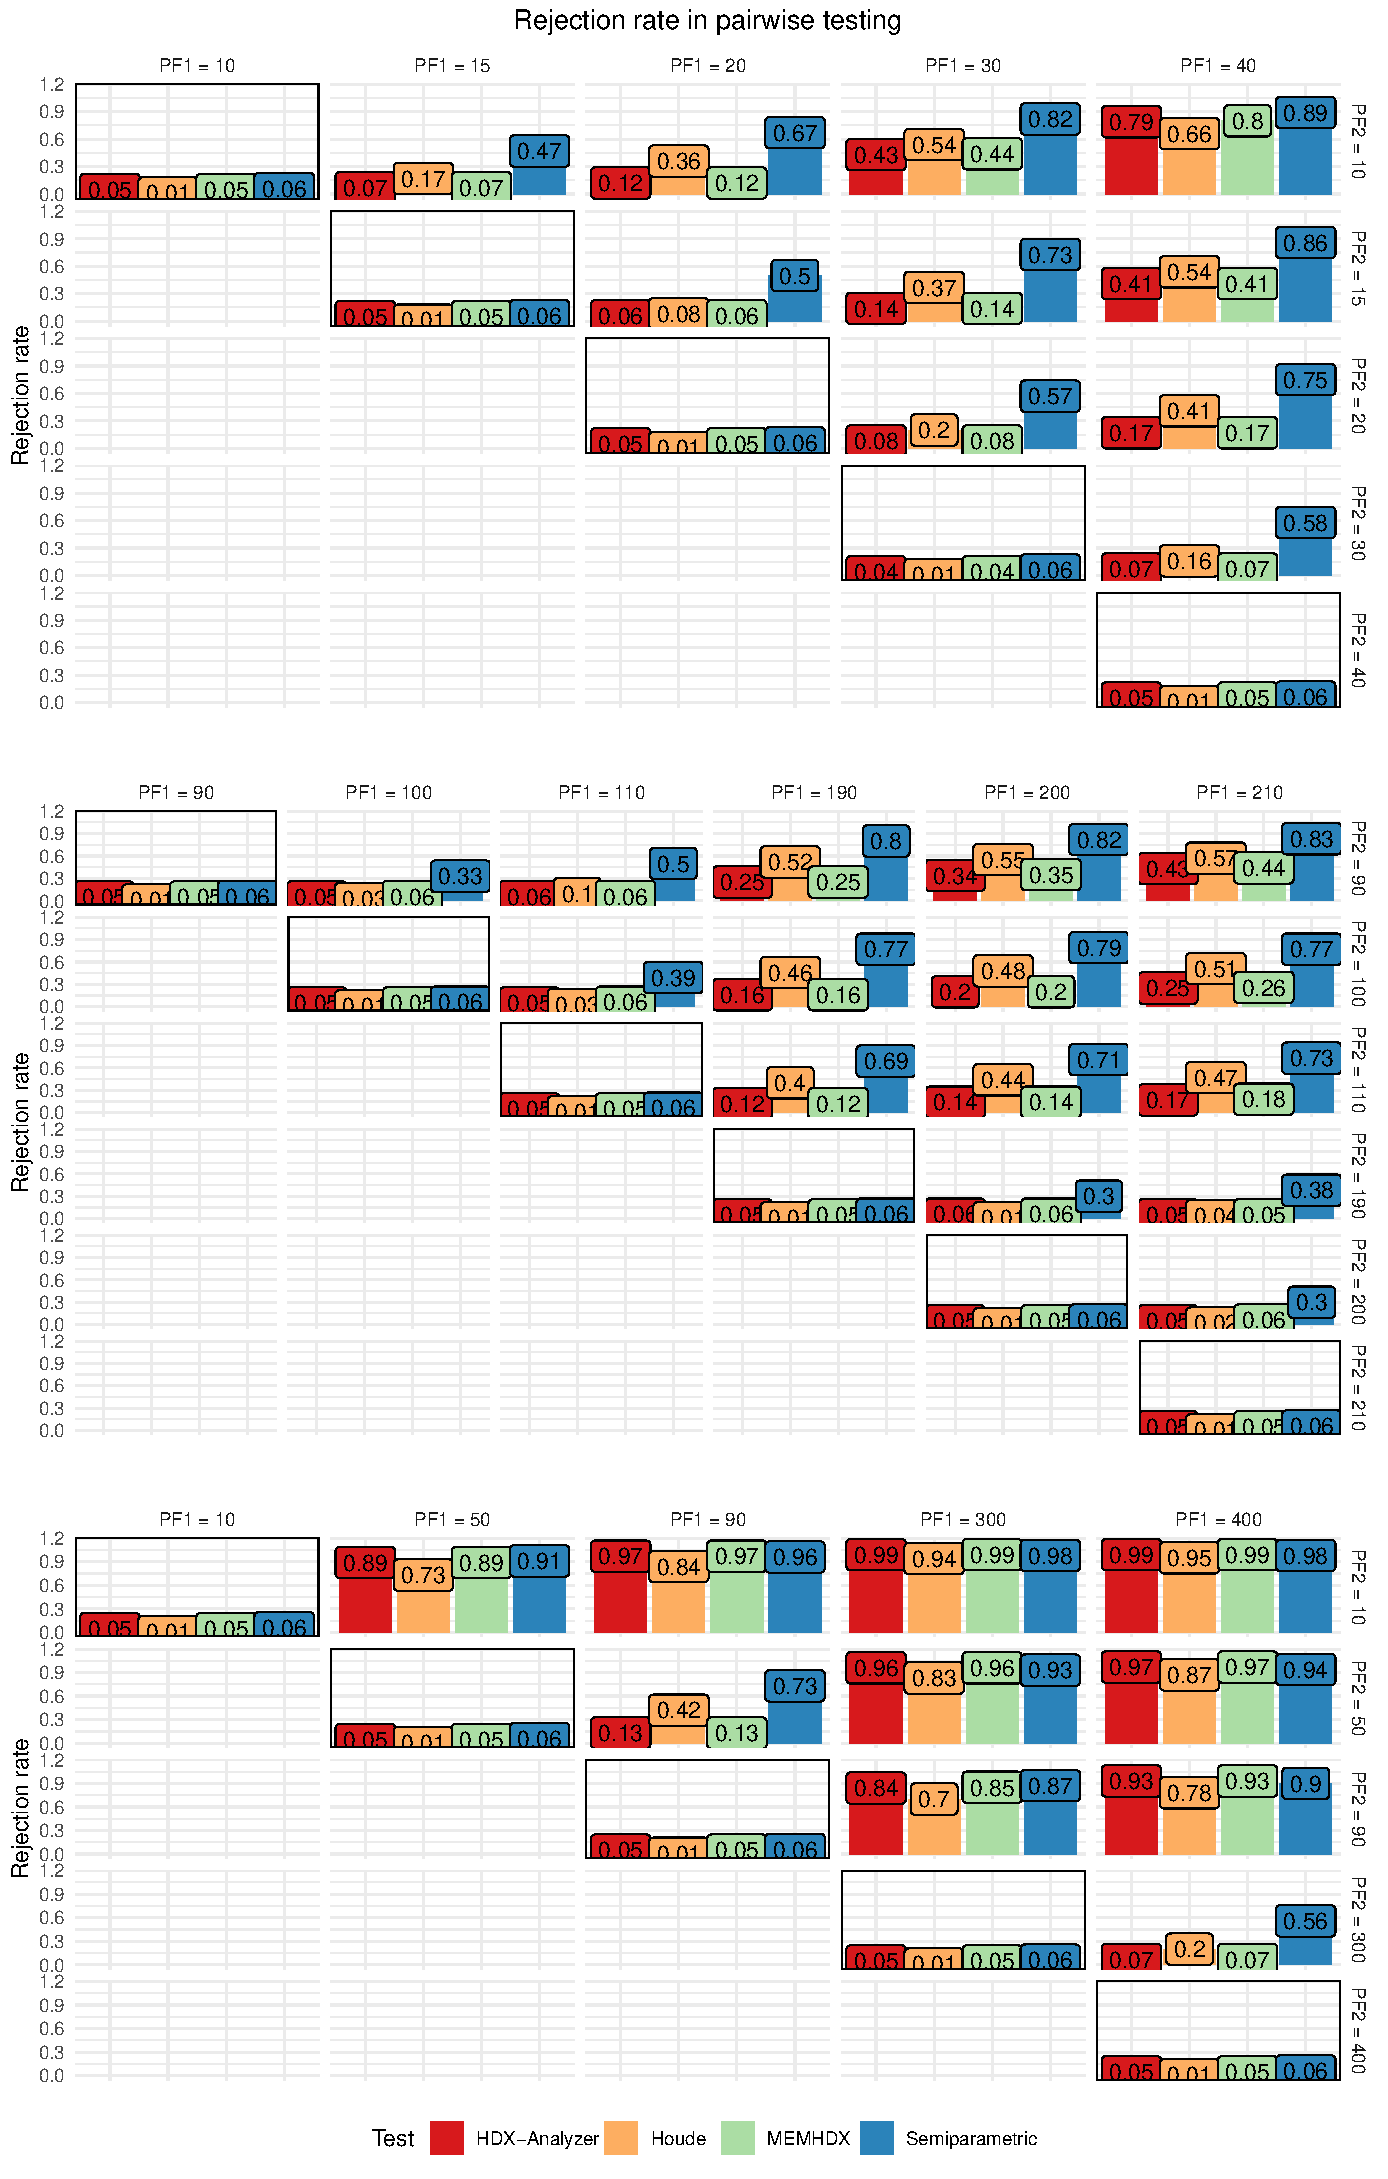
\includegraphics[width=0.95\textwidth]{Figures/results.pdf}
    \caption{Rejection rate in pairwise testing at the significance level $0.05$.}
\end{figure}


On the second plot we can see that the quality of the tests' performance decreases - we obtain fewer true rejections when compared to the first case. Houde's confidence intervals test generally fared better than the other existing methods. However, in the case when $\Delta Pf = 10$ the rejection rate is close to zero for all of the three approaches. The semiparametric test handle this difficult case better. The results are equal to about $30\%$.



The last plot presents the case when the differences between the protection factors $\Delta Pf$ are big. As we can see, the case when $Pf_1 = 300$ and $Pf_2 = 400$ turned out to be problematic for the existing approaches. The spline model fared better there. We can see the similar situation for $Pf_1 = 90$ and $Pf_2 = 50$. However, in this case, confidence intervals reached better results than before. For other pairs of protection factors, we observe an increase in the rate of true rejections. The values generally fluctuate between $85$ and $100\%$ except for Houde's test which turned out to be the worse.





\paragraph{Conclusions}

The performance of linear models leaves a lot to be desired. It is not surprising as the greatest variability of the values of deuterium uptake occurs during the short exposure. Since both HDX-Analyzer (estimated by OLS) and MEMHDX (estimated by MME) are sensitive to outliers we expect them to fit more the measurements of masses obtained using long incubation. The methods of robust regression such as Huber or bisquare weighting (in the case of HDX-Analyzer) may improve the results there.

The fact that the performance of Houde's test is better than the performance of the linear models can be also intuitively explained. Unlike other existing approaches, Houde's confidence intervals test takes into account the variability (averaged over time) of deuterium uptake along with the differential values. However, it is not surprising that its performance is poor in the case of close protection factors and that the test becomes quite conservative - averaging the differences over all the time points yields lower precision.

The regression spline model is not as exposed to the impact of outliers as HDX-Analyzer and MEMHDX (although it depends on the number of knots) because of its local characteristics. Thus, it is capable of modeling the deuterium uptake reasonably well along the entire curve. Moreover, the effects associated with the subjects and exposure time are modeled. It makes the test more sensitive to the protein protection level changes even when the differences are imperceptible by a human. 

The versatility of the proposed model is sufficient to employ it in similar problems, for example deuterium-hydrogen exchange (when we monitor the exact opposite of the HDX) or global HDX (when we focus on the whole protein instead of peptides). Therefore, we hope that our semiparametric model will be a valuable contribution to still too limited array of tools necessary to properly analyze results of HDX-MS 


 

\section{References}
\nocite{*}
\begin{filecontents}{\jobname.bib}
% Poniżej proszę wpisać pozycje bibliograficzne tak jak w plikach BibTeX (*.bib)



\end{filecontents}


\bibliographystyle{abbrv}
\bibliography{bibliography}


\bigskip
\setcounter{section}{0}
\selectlanguage{polish}
\Polskitrue
\subjclass{62J05; 92D20}
\keywords{deuteracja, wymiana izotopowa wodoru na deuter, spektrometria mas, HDX-MS, model semiparametryczny}

%\newpage
\begin{center}
{\bf Model semiparametryczny dla danych dotyczących wymiany izotopowej wodoru na deuter monitorowanej spektrometrią mas.}\\ 


\end{center}
\medskip

\begin{abstract}
Wymiana wodór-deuter monitorowana spektrometrią mas (HDX-MS) jest jedną z metod badania dynamiki i ukształtowania struktury białek. Podczas inkubacji w ciężkiej wodzie (D2O) reszty aminokwasowe bardziej wystawione na wymianę wodoru na deuter przechodzą ją znacznie szybciej niż inne. Pomiary mas peptydów ujawniają trwałość sieci wiązań wodorowych i regiony z ograniczoną dostępnością rozpuszczalnika. Szybkość wymiany może zależeć od stanu biologicznego białka (np. z lub bez obecnością ligandu) tzn. możebyć powiązana ze zmianami w ukształtowaniu jego struktury. W tym artykule proponujemy test opierający się na mieszanym modelu semiparametrycznym i regresji grzbietowej, który pozwala na dokładną identyfikację peptydów z istotne różnymi prędkościami wymiany w różnych stanach biologicznych. W celu oceny wyników testu, porównaliśmy go z innymi metodami służącymi do analizy danych z eksperymentów HDX-MS.
\end{abstract}

\begin{minipage}{0.2\textwidth}
        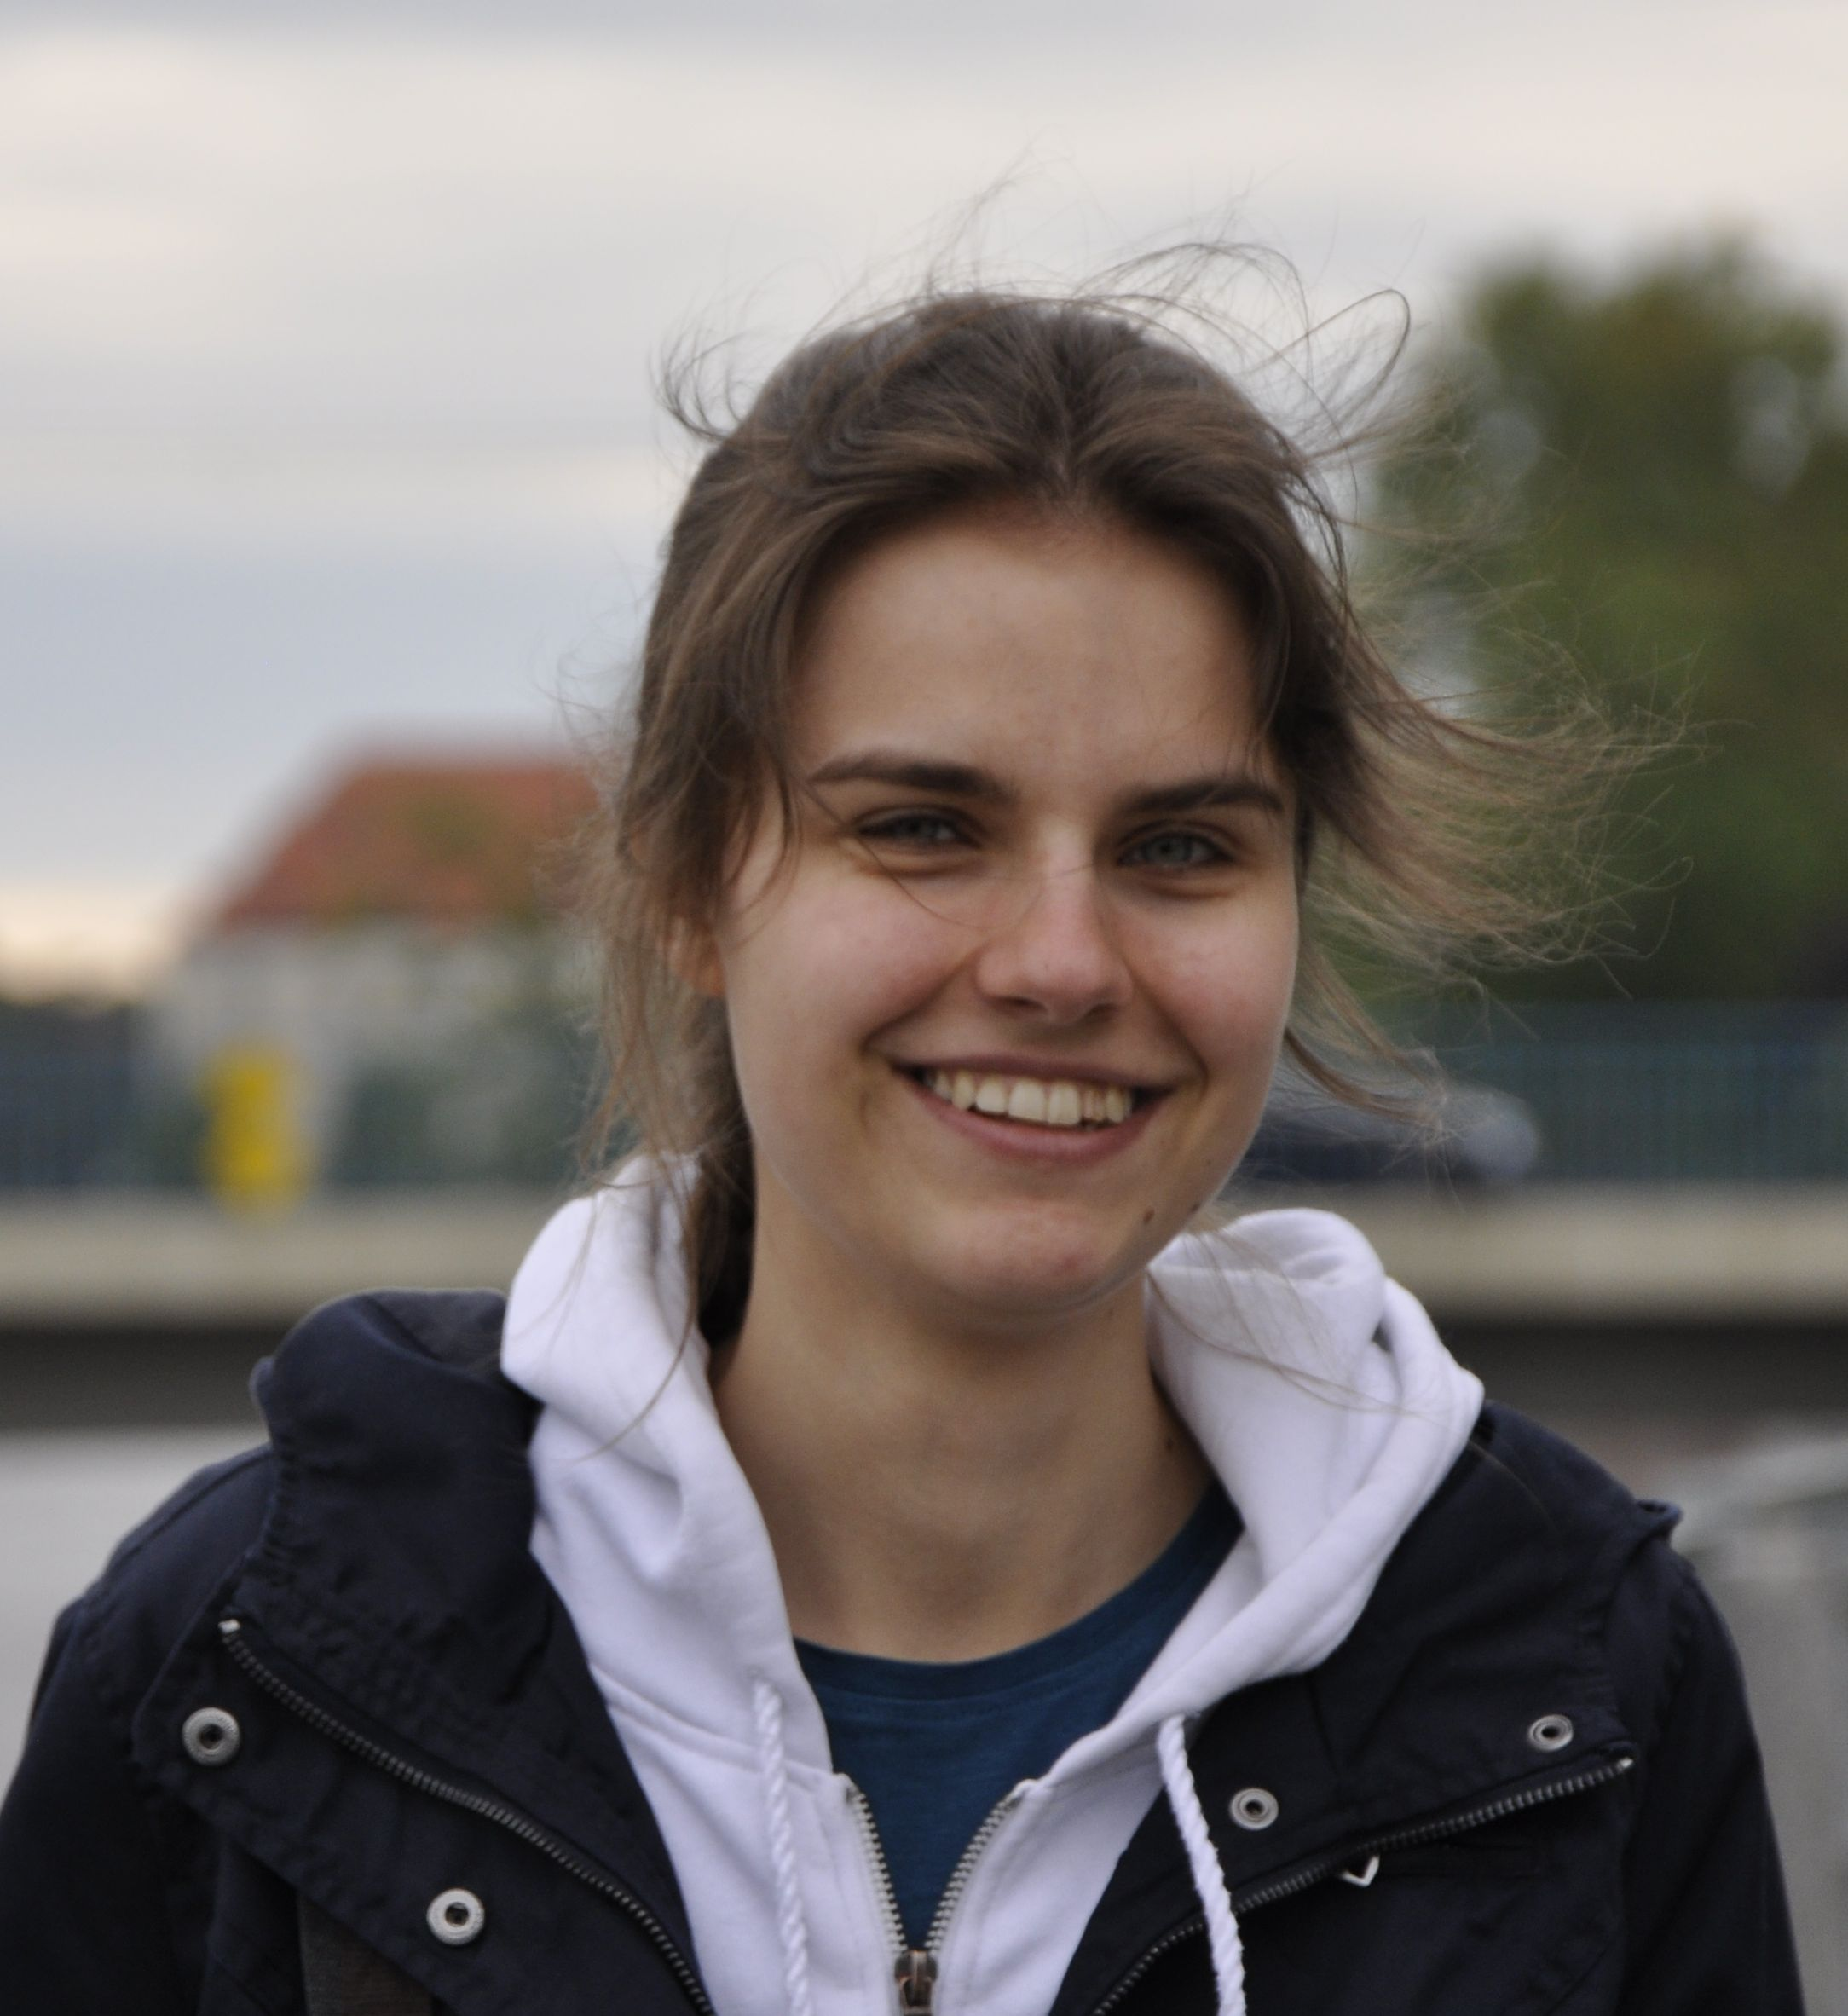
\includegraphics[width=1\textwidth]{Figures/Krystyna.JPG}
\end{minipage}
\hspace{0.01\textwidth}
\begin{minipage}{0.7\textwidth}
    Krystyna Grzesiak has completed her  M.Sc Mathematics with the Data Analysis specialization at the University of Wroclaw. She defended her master's thesis in 2021 under the supervision of doctor Michał Burdukiewicz and professor Małgorzata Bogdan. 
\end{minipage}

\begin{minipage}{0.2\textwidth}
        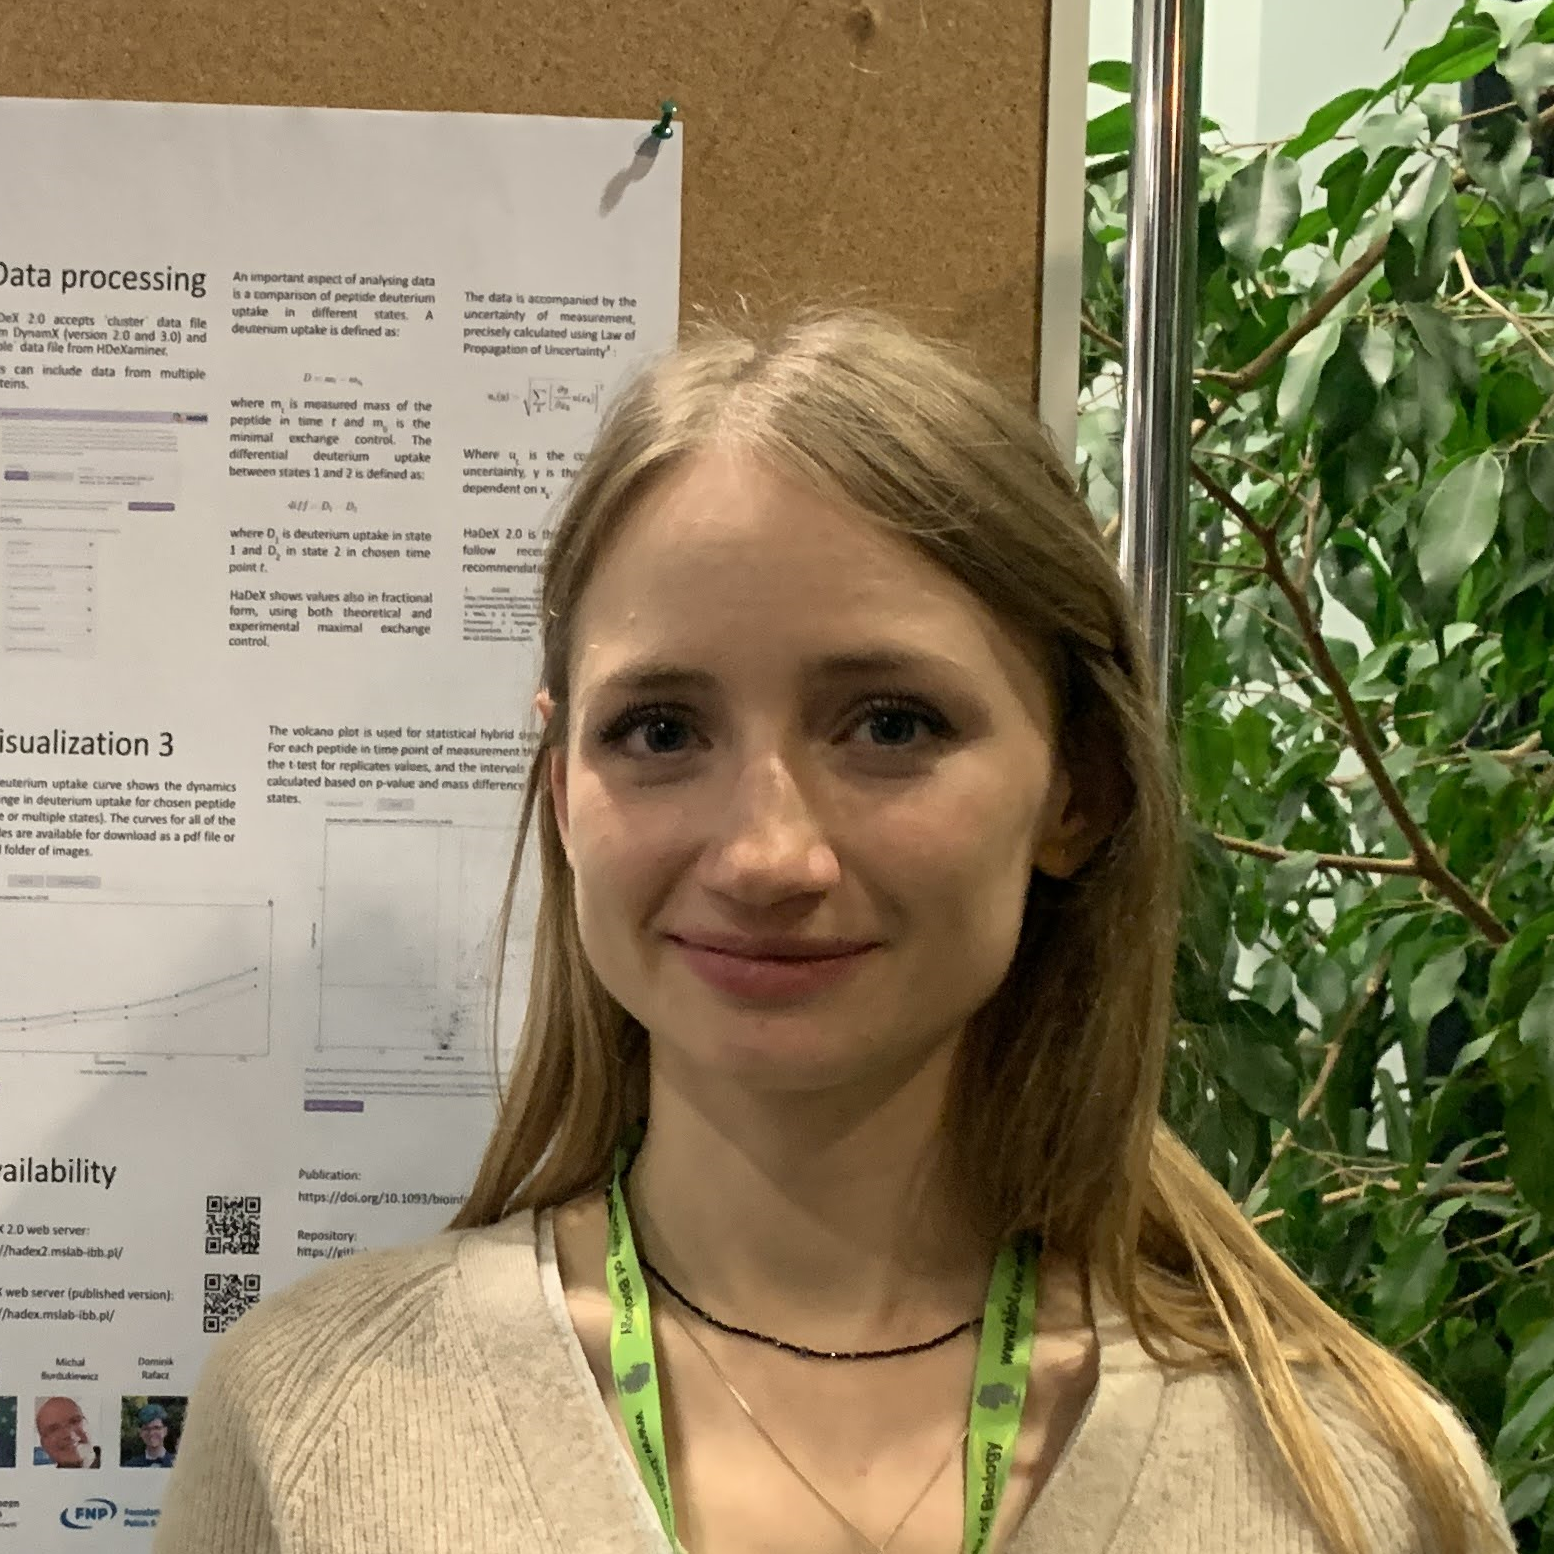
\includegraphics[width=1\textwidth]{Figures/weronika.png}
\end{minipage}
\hspace{0.01\textwidth}
\begin{minipage}{0.7\textwidth}
    Weronika Puchała is a physicist persuading her career in science in the field of biohysics and proteomics in the Dadlez Lab. Her PhD project is focused on the analysis of HDX-MS data. She is the main developer of the HaDeX software.
\end{minipage}

\begin{minipage}{0.2\textwidth}
        
\includegraphics[width=1\textwidth]{Figures/dadlez.jpg}
\end{minipage}
\hspace{0.01\textwidth}
\begin{minipage}{0.7\textwidth}
    Michał Dadlez is the head of the Mass Spectrometry Laboratory at Institute of Biochemistry and Biophysics PAS since 2001. His scientific interests include proteomics (with a focus on structural proteomics) and metabolomics, including small-molecule quantification.
\end{minipage}

\begin{minipage}{0.2\textwidth}
        
\includegraphics[width=1\textwidth]{Figures/Gosia.jpg}
\end{minipage}
\hspace{0.01\textwidth}
\begin{minipage}{0.7\textwidth}
Małgorzata Bogdan is an Associate Professor at the Institute of of Mathematics of Wroclaw University and Guest Professor at University of Lund. She is interested in the analysis of high dimensional data and its applications in statistical genetics.
\end{minipage}

\begin{minipage}{0.2\textwidth}
        
\includegraphics[width=1\textwidth]{Figures/michal.jpeg}
\end{minipage}
\hspace{0.01\textwidth}
\begin{minipage}{0.7\textwidth}
Michał Burdukiewicz is a research assistant in the Centre for Clinicial Research at Medical University of Bia\l{}ystok. His research interests cover applications of machine learning in functional analysis of peptides and proteins and proteomics, especially hydrogen-deuterium exchange monitored by mass spectrometry.
\end{minipage}

\Koniec
\end{document}
